\chapter{One Algorithm, Three Machines}
\label{ch:three-machines}

A memory region contains words. We want one word that summarizes them: load
each word, combine it with an accumulator by exclusive OR, and return the
accumulator. The routine is small enough to trace on paper. It is large enough
to bring together almost every distinction in this book: words and their
readings, byte-addressed memory, effective addresses, loops, observations,
calling conventions, cross-machine relations, and evidence that can fail.

The three programs will run on A0, RV64I, and x86-64. ``The same algorithm''
will not mean that their registers have the same names or that their traces
have the same number of steps. It will mean that each program satisfies one
mathematical contract and that explicit relations connect their states to that
contract.

\begin{keyidea}[title={One specification, three different movements}]
We do not prove that the instruction sequences look alike. We prove that each
sequence consumes the same logical input region and returns the same XOR
reduction, while respecting its own machine and calling contract.
\end{keyidea}

\section{Why reduction algorithms matter}

A \keyterm{reduction} combines a sequence into one result. Addition produces a
sum. Minimum keeps the least element. Conjunction asks whether every Boolean
value is true. Exclusive OR records whether each bit position appeared an odd
or even number of times. Reductions appear in checksums, statistics, database
aggregation, parallel programs, cryptographic constructions, and the inner
loops of scientific codes.

Long before a compiler could translate such a loop automatically, programmers
had to decide where the accumulator lived, how a pointer advanced, and how an
end condition was represented. Modern processors make the same movement at a
larger scale. Vector and parallel reductions combine many elements at once,
then merge partial accumulators. Those faster forms raise questions about
ordering, associativity, floating-point rounding, and optional extensions. We
begin with the scalar integer case because its complete meaning fits on the
page.

Exclusive OR is a particularly clean teaching operation. For words of one
fixed width it is associative and commutative:
\[
 (x\mathbin{\mathsf{xor}}y)\mathbin{\mathsf{xor}}z
 =x\mathbin{\mathsf{xor}}(y\mathbin{\mathsf{xor}}z),
 \qquad
 x\mathbin{\mathsf{xor}}y=y\mathbin{\mathsf{xor}}x.
\]
Zero is its identity, and every word cancels itself:
\[
 x\mathbin{\mathsf{xor}}0=x,
 \qquad x\mathbin{\mathsf{xor}}x=0.
\]
These laws explain the loop invariant without hiding any overflow convention.
XOR acts independently at every bit position and always returns another word
of the same width.

This routine is not a cryptographic hash. Reordering the input words leaves
the result unchanged, and equal words cancel in pairs. The example is useful
because its weakness is visible: it teaches a machine proof, not a security
claim.

That distinction has a historical analogue. Simple parity and longitudinal
redundancy checks were attractive because a human or a small circuit could
update them while data moved. They detected selected transmission faults with
little state. Their algebra also admitted undetected patterns. Stronger cyclic
codes and later cryptographic hashes were developed for stronger fault and
adversary models. Hamming's foundational treatment makes the central design
question explicit: which error patterns a code can detect or correct
\autocite{hamming1950codes}. The lesson is not that XOR is obsolete. It is that an
operation earns meaning from its contract: the same reduction can be a useful
diagnostic checksum, a reversible mask component, or a dangerously weak
authenticator.

Our contract asks only for the reduction value. It does not say that unequal
regions have unequal reductions, that a changed word is always detected, or
that an attacker cannot preserve the result. Keeping those tempting claims out
of the theorem is part of formal precision. It also demonstrates why proof
does not rescue a poor specification: a flawless implementation proof can
establish exactly the weak property that was requested.

\section{The contract before the code}

Fix width 64. Let \(M\) be byte-addressed memory, \(a\) the starting address,
and \(n\) an unsigned count. Define the little-endian word load from Chapter 4
as \(L(M,q)\). The desired result is
\[
 \mathop{\mathsf{foldxor}}(M,a,n)
 = L(M,a)\mathbin{\mathsf{xor}}L(M,a+8)
   \mathbin{\mathsf{xor}}\cdots
   \mathbin{\mathsf{xor}}L(M,a+8(n-1)),
\]
with value zero when \(n=0\).

Ellipsis is convenient prose but a poor base definition. The recursive form
names both cases exactly:
\[
 \begin{array}{rcl}
 \mathop{\mathsf{foldxor}}(M,a,0)&=&0,\\
 \mathop{\mathsf{foldxor}}(M,a,n+1)&=&
   L(M,a)\mathbin{\mathsf{xor}}
   \mathop{\mathsf{foldxor}}(M,a+8,n).
 \end{array}
\]

The program contract needs more than this equation. Each of the \(n\) loads
must be valid. Address formation must not wrap around the 64-bit address
space. The code region must be executable under the selected machine model.
The calling convention must place the pointer and count where the listing
expects them. On normal return, the result register must equal
\(\mathop{\mathsf{foldxor}}(M,a,n)\), and memory must be unchanged.

\begin{definition}[title={XOR-reduction call contract}]
The input consists of an initial memory \(M_0\), address \(a\), and count
\(n\). The precondition requires every range \([a+8i,a+8i+8)\), for
\(0\le i<n\), to be readable and requires the address calculations not to
wrap. Normal return must preserve \(M_0\) and place
\(\mathop{\mathsf{foldxor}}(M_0,a,n)\) in the declared result register.
The contract observes normal return, the result word, and memory preservation.
\label{def:xor-reduction-contract}
\end{definition}

\begin{figure}[htbp]
\centering
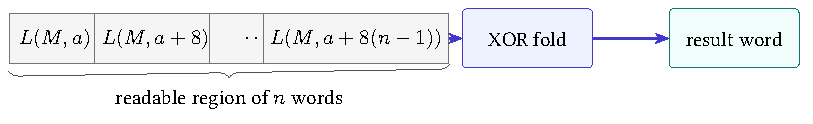
\includegraphics[width=0.92\textwidth]{figures/xor-reduction-contract}
\caption{The contract connects a logical region of \(n\) words to one result.
Pointer motion and accumulator updates are implementation details.}
\figalt{A row of memory words enters an XOR fold and produces one result word; a bracket names the readable input region.}
\label{fig:xor-reduction-contract}
\end{figure}

The contract deliberately permits \(n=0\). In that case the readable region
is empty, no load occurs, and the result is zero. The address \(a\) need not be
readable because no byte at that address is accessed. A precondition that
always demanded eight readable bytes would be stronger than the routine needs.

Alignment is separate. Core A0 permits a word access to begin at any address
provided the full byte range exists. The selected RV64I environment may trap
or handle a misaligned load outside the base instruction semantics, depending
on its execution environment. The selected x86-64 form permits an unaligned
ordinary load in this model. For one clean three-way theorem, we require
\(a\) to be divisible by eight. This is a theorem premise chosen for the
relation, not a universal statement about all three machines.

\begin{warning}[title={A valid first address does not validate the region}]
Checking \(a\) alone is insufficient. The final access begins at
\(a+8(n-1)\), and all eight of its bytes must exist. The no-wrap and range
premises quantify over every iteration.
\end{warning}

\section{The language-independent loop}

The algorithm carries four logical values: the original memory \(M_0\), the
number \(i\) of words already consumed, the current pointer \(p=a+8i\), and
the accumulator
\[
 x=\mathop{\mathsf{foldxor}}(M_0,a,i).
\]
It also carries a remaining count \(c=n-i\). The following \keyterm{pseudocode}
is a readable algorithm sketch rather than an executable language:

\begin{codelisting}[language={},caption={The logical XOR-reduction loop}]
p := a
c := n
x := 0
while c != 0:
    x := x xor load64(M, p)
    p := p + 8
    c := c - 1
return x
\end{codelisting}

The order of the three body updates matters to a step-by-step proof even though
the final mathematics is simple. The load uses the old pointer. The
accumulator gains word \(i\). The pointer then names word \(i+1\), and the
remaining count becomes \(n-(i+1)\).

\begin{definition}[title={Loop invariant}]
At the test before iteration \(i\), where \(0\le i\le n\), memory equals
\(M_0\), the pointer equals \(a+8i\), the remaining count equals \(n-i\), and
the accumulator equals \(\mathop{\mathsf{foldxor}}(M_0,a,i)\).
\label{def:xor-loop-invariant}
\end{definition}

\begin{figure}[htbp]
\centering
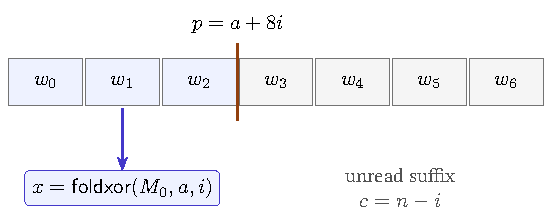
\includegraphics[width=0.9\textwidth]{figures/xor-loop-invariant}
\caption{The invariant cuts memory into a consumed prefix and an unread suffix.
The accumulator summarizes exactly the prefix.}
\figalt{A memory row is divided at pointer p; the left i words feed the accumulator and the right n minus i words remain.}
\label{fig:xor-loop-invariant}
\end{figure}

\begin{proofkit}[title={Reader proof of the logical loop}]
\textbf{Initialization.} Before the first test, \(i=0\). The pointer is \(a\),
the count is \(n\), memory is unchanged, and the accumulator is zero. These
are exactly the four invariant clauses because the reduction of an empty
prefix is zero.

\textbf{Preservation.} Assume the invariant at a test with \(c\ne0\). Then
\(i<n\), so the precondition makes \(L(M_0,a+8i)\) valid. The load reads that
word without changing memory. XOR changes the accumulator to
\[
 \mathop{\mathsf{foldxor}}(M_0,a,i)
 \mathbin{\mathsf{xor}}L(M_0,a+8i)
 =\mathop{\mathsf{foldxor}}(M_0,a,i+1).
\]
The pointer addition produces \(a+8(i+1)\), and decrement produces
\(n-(i+1)\). Thus the invariant holds for the next test.

\textbf{Exit.} If the test sees \(c=0\), the invariant gives \(n-i=0\), hence
\(i=n\). The accumulator is therefore
\(\mathop{\mathsf{foldxor}}(M_0,a,n)\), memory still equals \(M_0\), and the
return value satisfies the contract.

\textbf{Termination.} The remaining count is a natural number. Every body
execution begins with a positive count and decreases it by one without
wraparound. It therefore reaches zero after exactly \(n\) iterations.
\end{proofkit}

This proof has two parts that bounded testing cannot replace. Preservation is
quantified over every legal iteration, and termination covers every natural
input count admitted by the contract. Testing can still find mistakes in an
implementation or in the connection between its registers and these logical
variables.

\section{From an algorithm to a machine theorem}

The pseudocode is not an instruction-set-neutral executable. Its word
\code{load64} already assumes an address unit, byte order, access width, and
failure policy. Its subtraction assumes a positive remaining count. Its return
assumes an interface with a caller. Lowering the loop means discharging
obligations, not replacing words with mnemonics.

First comes \keyterm{representation}. Each logical variable needs a machine
location at each cut point. The accumulator may remain in one register. The
pointer and count may be overwritten because the contract observes their
initial values and final result, not their final register contents.

Second comes \keyterm{operation refinement}. A machine load must reconstruct
\(L(M,p)\). XOR must implement bitwise exclusive OR at width 64. The pointer
update must represent addition by eight without wrapping on admitted inputs.
The count update must represent natural-number subtraction by one. The branch
must continue exactly when the new count is nonzero.

Third comes \keyterm{control refinement}. Setup reaches the first loop cut
point. One body path reaches the next cut point. The zero-count path reaches a
successful terminal observation. Invalid fetches, loads, or returns must not
be relabeled as success. Program-counter equations differ, but this shape is
shared.

Fourth comes \keyterm{frame preservation}: state outside the allowed write set
remains unchanged. Memory is the main frame component here. ABI-preserved
registers and stack state join it for the real-machine versions that a caller
can invoke as procedures. A
result equation alone would miss both forms of damage.

\begin{table}[htbp]
\centering
\caption{The lowering obligations carried by every listing.}
\begin{tabular}{@{}p{0.2\textwidth}p{0.7\textwidth}@{}}
\toprule
Obligation & Required connection \\
\midrule
Representation & registers and memory correspond to \(p,c,x,M_0\) \\
Operation & load, XOR, add, and decrement implement the logical body \\
Control & setup, body, exit, and outcome follow the loop structure \\
Frame & memory and protected procedure state remain unchanged \\
Encoding & fetched bytes decode to the instruction instances in the proof \\
\bottomrule
\end{tabular}
\end{table}

The last row is easy to omit when reasoning from assembly text. A proof of the
mnemonic sequence is not yet a proof about executable bytes. The final artifact
must bind assembled bytes, instruction boundaries, decoded operands, and the
semantic instances used by the step relation. This chapter prints readable
assembly because those decoders do not yet exist in Axeyum; that absence stays
visible in the evidence boundary.

\begin{tryit}[title={Build the cut-point map first}]
For each listing below, mark entry, the first state satisfying \(B_0\), the
load state, the next loop-head state, and the successful terminal state. Write
which logical variables are meaningful at each mark.
\end{tryit}

\section{A0 makes the proof state visible}

Use width-64 A0 with the following entry convention: \(r_1=a\), \(r_2=n\),
and memory \(M_0\). Register \(r_0\) is the result. Registers \(r_3,r_4,r_5\)
are scratch. The listing uses labels for reading; encoding replaces each label
with the signed displacement defined in Chapter 9.

\begin{codelisting}[language={},caption={A0 XOR reduction}]
00: movi      r0, 0
04: movi      r4, 8
08: movi      r5, 1
0c: cmp       r2, r0
10: branch.eq done
loop:
14: load      r3, [r1+0]
18: xor       r0, r0, r3
1c: add       r1, r1, r4
20: sub       r2, r2, r5
24: branch.ne loop
done:
28: halt
\end{codelisting}

The first comparison handles the empty input without loading. The subtraction
sets A0's zero condition from the new count, so the backward branch can reuse
that result. The XOR also changes conditions, but the later subtraction
overwrites them before \code{branch.ne}. This ordering is a small live-state
argument: the branch depends on conditions from \code{sub}, not conditions
from \code{xor}.

At the loop head, relate \(r_1\) to \(p\), \(r_2\) to \(c\), and \(r_0\) to
\(x\). Registers \(r_4=8\) and \(r_5=1\) are fixed helpers. The A0 state also
contains the program counter, condition bits, outcome, program bytes, and
memory. The invariant does not erase these components. It constrains those
needed for the proof and permits the current condition bits to have whatever
values the preceding legal path produces.

The backward branch begins at byte address 36 and targets byte address 20.
A0's rule is \(p+4+4d\), so
\[
 36+4+4d=20,
\]
which gives \(d=-5\). The forward branch at address 16 targets address 40 and
therefore uses \(d=5\). Both fit the signed byte field.

\begin{example}[title={A complete two-word A0 trace at loop granularity}]
Let \(n=2\), let the first word be \(u\), and let the second be \(v\). At the
first loop head, \((r_1,r_2,r_0)=(a,2,0)\). After one body,
\((r_1,r_2,r_0)=(a+8,1,u)\). After the second body,
\((r_1,r_2,r_0)=(a+16,0,u\mathbin{\mathsf{xor}}v)\). The second backward
branch is not taken. Execution reaches \code{halt} with the required result.
\end{example}

This summary suppresses the instruction-level intermediate states. A machine
trace must retain them: the state after the load, the state after XOR, both
arithmetic updates, and the branch successor. The loop-granularity relation
holds at selected cut points, not after every instruction.

\subsection{A0 failure controls}

Four small mutations test different obligations. Change the load displacement
from zero to eight; the first iteration skips the first word. Change the
pointer increment from eight to one; the next load overlaps the first word.
Change the decrement helper from one to zero; termination fails. Change the
backward displacement from \(-5\) to \(-4\); control returns to the XOR rather
than the load, reusing stale \(r_3\). Each mutation should produce a distinct
counterexample or control-flow failure.

For the empty case, poison the bytes at \(a\) or make the address unreadable.
The valid program must still halt normally with zero because it never loads.
That control distinguishes a true zero-iteration path from an implementation
that reads once.

\section{RV64I carries the predicate in registers}

Use the standard integer calling names for exposition: \code{a0} initially
holds \(a\), \code{a1} holds \(n\), and \code{a0} carries the return value.
Because the pointer and result share \code{a0} at different times, copy the
pointer to temporary \code{t0} before clearing the accumulator.

\begin{codelisting}[language={},caption={RV64I XOR reduction}]
    addi t0, a0, 0
    addi a0, x0, 0
    beq  a1, x0, done
loop:
    ld   t1, 0(t0)
    xor  a0, a0, t1
    addi t0, t0, 8
    addi a1, a1, -1
    bne  a1, x0, loop
done:
    jalr x0, 0(ra)
\end{codelisting}

Every instruction belongs to the base integer slice used by this book
\autocite{riscv2026unpriv}. The
\code{addi} forms perform copying, zero construction, pointer advance, and
count decrement. The conditional branches compare \code{a1} directly with
the architectural zero register. No arithmetic flags exist in the selected
state. The final \code{jalr} returns through the incoming link register under
the calling convention discussed in Chapter 10.

At the RV64 loop head, \code{t0} represents \(p\), \code{a1} represents
\(c\), and \code{a0} represents \(x\). Temporary \code{t1} is unconstrained
before the load and equals the current word afterward. The state relation must
also say that the address translation used by memory is identity on the input
region, or state another explicit mapping.

The instruction \code{ld} forms an effective address from \code{t0} plus the
sign-extended immediate zero and reconstructs a 64-bit little-endian value.
The pointer increment is modulo \(2^{64}\), but the contract's no-wrap premise
makes its mathematical reading equal to \(a+8(i+1)\). Likewise, decrement is
modular machine arithmetic; the loop guard and invariant ensure it is applied
only to a positive count.

\begin{sidebar}[title={The proof uses the ABI without confusing it with the ISA}]
The ISA gives meanings to integer-register numbers, \code{ld}, branches, and
\code{jalr}. The ABI gives the names \code{a0}, \code{a1}, \code{t0},
\code{t1}, and \code{ra}, and states which registers a caller may expect to
survive. Both layers are needed for a callable routine. They are different
sources of obligations.
\end{sidebar}

The listing changes \code{a1}, \code{t0}, and \code{t1}. Under the selected
calling convention these are caller-saved registers. It does not adjust the
stack or call another routine. Its memory action is read-only. A correctness
statement at ISA level can ignore ABI preservation; the callable-routine
theorem cannot.

\section{x86-64 lets the loop reuse status flags}

Under the selected System V integer convention, \code{rdi} holds \(a\),
\code{rsi} holds \(n\), and \code{rax} carries the result. This Intel-syntax
listing uses only scalar integer instructions.

\begin{codelisting}[language={},caption={x86-64 XOR reduction}]
    xor  eax, eax
    test rsi, rsi
    je   done
loop:
    xor  rax, qword ptr [rdi]
    add  rdi, 8
    sub  rsi, 1
    jne  loop
done:
    ret
\end{codelisting}

Writing \code{eax} clears all of \code{rax} in 64-bit mode
\autocite{intel2026sdm1}. This is a selected
x86-64 subregister rule, not a generic property of narrow writes. The
\code{test} instruction computes a logical conjunction for flags without
storing the result. Here it sets the zero flag exactly when the count is zero.
The memory-source XOR loads a 64-bit word and combines it with the accumulator.
The subtraction sets the zero flag from the new count, and \code{jne} consumes
that flag.

At the loop head, \code{rdi} represents \(p\), \code{rsi} represents \(c\),
and \code{rax} represents \(x\). The relevant status-flag values are those
created by the path into the head. The cross-machine relation need not equate
x86 status flags with RV64 state because RV64 has no corresponding component.
It must ensure that each machine chooses the same logical exit condition at
the compared cut points.

The listing mutates \code{rdi} and \code{rsi}. They are caller-saved under the
selected ABI, as is \code{rax}. The routine preserves the stack pointer and
callee-saved registers and returns through the address already on the stack.
These facts are not visible in the mathematical fold equation, but they are
part of the procedure contract.

\begin{warning}[title={Equivalent results can hide unequal fault behavior}]
If the readable-region premise is removed, the three programs need not fail in
the same way. Alignment policy, address translation, and fault delivery differ.
Our theorem relates normal executions under the printed precondition. It does
not assert universal agreement for invalid memory.
\end{warning}

\section{Local lemmas beneath the simulation}

The three-machine proof kit below compresses many instruction facts into one
body paragraph. A formal development should expose them as small lemmas. The
load lemma starts from related pointers and memory and ends with equal loaded
words. It depends on effective-address formation, range validity, access width,
and little-endian reconstruction. It says nothing yet about the accumulator.

The combine lemma starts from equal logical accumulator values and equal
loaded words. It concludes that the three destination words agree after XOR.
A0 and x86 also update condition state; RV64I does not. Those side effects are
allowed by the relation but must be described because later control may
observe them.

The pointer lemma connects three modular additions to the ordinary equality
\(p'=p+8\). Its proof uses the no-wrap premise. The decrement lemma connects
machine subtraction to \(c'=c-1\) and uses \(c>0\). The control lemma then
shows that the A0 zero condition, RV64 register comparison, and x86 zero flag
select continuation exactly when \(c'\ne0\).

These lemmas meet in a deliberate order. Proving the branch before showing
which instruction last wrote its condition state would leave a gap. Proving
the load without the address relation would compare bytes from different
locations. Proving arithmetic only as a word equality would not justify the
natural-number decrease used for termination.

\begin{sidebar}[title={Small lemmas localize a counterexample}]
A load mismatch points toward address or memory semantics. An equal load
followed by unequal accumulators points toward XOR or register writes. Equal
body values followed by unequal paths points toward conditions or targets.
\end{sidebar}

One may also prove each machine correct against the logical loop separately
and derive pairwise agreement by transitivity. That structure often scales
better than one ternary relation. The direct three-way presentation keeps the
shared cut points visible. An Axeyum implementation may store one
machine-to-logical simulation per architecture and construct its comparison
report from their common logical observations.
\section{Relating three traces}

The listings have different setup lengths and different numbers of
instructions per iteration. A lockstep relation would fail immediately. We
instead compare \keyterm{cut points}: entry, loop head, and normal return. One
logical body corresponds to several machine steps on every architecture, but
the number and placement of those steps need not agree.

\begin{figure}[htbp]
\centering
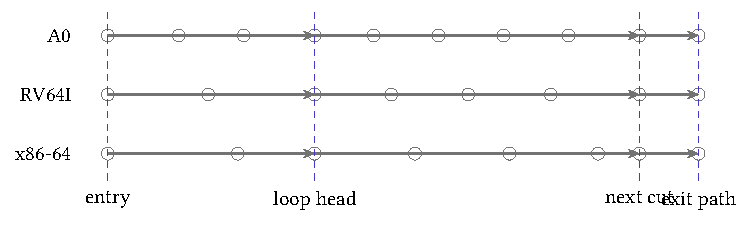
\includegraphics[width=0.94\textwidth]{figures/xor-three-traces}
\caption{Different instruction traces meet at common logical cut points. The
dashed bands represent initialization, one body, and exit.}
\figalt{Three horizontal traces labeled A0, RV64I, and x86-64 have unequal numbers of small steps between aligned entry, loop, and return bands.}
\label{fig:xor-three-traces}
\end{figure}

Define relation \(B_i\) at the loop head. It requires all three memories to
agree on the input region and to remain equal to \(M_0\). It maps A0 \(r_1\),
RV64 \code{t0}, and x86 \code{rdi} to \(a+8i\). It maps A0 \(r_2\), RV64
\code{a1}, and x86 \code{rsi} to \(n-i\). It maps A0 \(r_0\), RV64
\code{a0}, and x86 \code{rax} to the reduction of the first \(i\) words. It
also places each program counter at its own loop test or body cut point and
requires each machine to remain in normal execution.

\begin{proofkit}[title={Three-machine forward simulation}]
\textbf{Entry to first cut point.} Each setup sequence preserves memory,
copies or retains the input pointer, constructs the zero accumulator, and
retains the count. Therefore \(B_0\) holds.

\textbf{Body correspondence.} Assume \(B_i\) and \(i<n\). The three effective
addresses all denote \(a+8i\). By memory agreement and common little-endian
reconstruction, the loads return one word \(u=L(M_0,a+8i)\). Each accumulator
becomes its old value XOR \(u\). Each pointer advances by eight, and each count
decreases by one. The no-wrap and positive-count premises connect the modular
updates to ordinary arithmetic. Thus \(B_{i+1}\) holds at the next cut point.

\textbf{Exit correspondence.} Under \(B_i\), all three loop tests see zero
exactly when \(n-i=0\). They therefore exit together at the logical level,
although through different instructions. Then \(i=n\), and all three result
registers equal \(\mathop{\mathsf{foldxor}}(M_0,a,n)\). Their return mechanisms
establish the selected procedure observations.
\end{proofkit}

The proof composes two ideas. The loop invariant connects each implementation
to the mathematical fold. The cross-state relation connects corresponding
implementation cut points. Either route can be used alone, but together they
explain both correctness and agreement.

\subsection{What the relation intentionally forgets}

A0 condition bits, x86 status flags, and RV64 temporary values need not agree.
Instruction bytes and program counters differ. A0 ends through \code{halt} in
the pedagogical listing, whereas the two callable real-ISA listings return to
a continuation. A direct theorem between those terminal states must either
map A0 halt to a harness-defined return observation or give A0 a fixed-return
wrapper as described in Chapter 10.

The distinction is substantive. Without the harness, ``all three return'' is false
for the printed A0 program. The clean statement is that all three reach their
declared successful terminal observation with the same result. A later Axeyum
package should encode that observation rather than force unlike control states
to be equal.

\section{Execute a concrete instance}

Let \(a=256\), \(n=3\), and let the three loaded words be
\[
 u=\mathtt{0f0f},\qquad v=\mathtt{00ff},\qquad
 z=\mathtt{0ff0},
\]
shown with leading zeroes omitted. The successive accumulator values are
\[
 0,quad \mathtt{0f0f},quad \mathtt{0ff0},quad \mathtt{0000}.
\]
The pointer values at loop heads are 256, 264, 272, and 280. The remaining
counts are 3, 2, 1, and 0. The final zero is not evidence that no work
occurred; these particular words cancel.

\begin{table}[htbp]
\centering
\caption{The logical trace for the three-word example.}
\begin{tabular}{@{}rrrr@{}}
\toprule
\(i\) & pointer & remaining & accumulator \\
\midrule
0 & 256 & 3 & \code{0000} \\
1 & 264 & 2 & \code{0f0f} \\
2 & 272 & 1 & \code{0ff0} \\
3 & 280 & 0 & \code{0000} \\
\bottomrule
\end{tabular}
\end{table}

A useful test suite includes more than this attractive cancellation. Test an
empty input, one word, two unequal words, two equal words, a region near the
highest permitted address, and a pattern with high bits set. For each case,
compare the complete outcome class and memory, not only the result register.

\section{Breaking the proof on purpose}

Negative controls should target the binding chain from Chapter 14. At the
specification layer, change the fold identity from zero to all ones. At the
memory layer, reverse the byte order of one decoder. At the instruction layer,
change one pointer increment from eight to four. At the control layer, branch
on zero rather than nonzero after decrement. At the ABI layer, place the count
in the wrong entry register. At the observation layer, forget memory
preservation and introduce a store that the result-only comparison ignores.

Each control needs a small separating input. The empty input directly
separates the wrong identity. A two-word region with distinct halves exposes a
four-byte pointer increment. A count of one exposes an inverted continuation
branch. A count of zero exposes an implementation that loads before checking.
A memory snapshot before and after exposes the hidden store.

\begin{tryit}[title={Find the first separating iteration}]
Change the RV64 pointer update to \code{addi t0,t0,16}. For \(n=3\), write the
addresses loaded by the valid and mutated programs. Choose three word values
so that the first result disagreement occurs only after the second load.
\end{tryit}

Counterexamples should replay as traces. A solver assignment saying
\(n=2\) and giving two memory words is not yet an explanation. Decode the
program, execute both versions from the assigned state, and print the first cut
point where pointer, count, accumulator, outcome, or memory agreement fails.

\section{Cost questions come after correctness}

The three listings invite counting, but one number cannot settle which is
best. A0 uses fixed four-byte instructions and materializes constants in
registers. RV64I also uses fixed-width base instructions but has immediate
forms and a zero register. x86-64 uses variable-length encodings and a
memory-source XOR. Instruction counts, encoded bytes, decoded operations,
loads, branches, and estimated cycles are different costs.

For a positive count, every listing executes its setup and entry test, one
load and combine per word, pointer and count updates, and a continuation test.
The final not-taken branch is still an executed instruction. Symbolic dynamic
counts can be derived from the listings, but they describe abstract paths, not
processor timing. Caches, prediction, instruction fusion, and other
microarchitectural facts are outside the scalar ISA model.

Code-byte comparison requires actual encodings. The x86 memory-source form may
save a separately decoded load while using more bytes for other instructions.
RV64 compressed encodings would change byte cost, but the optional compressed
extension is outside this chapter's language. Admitting it for one candidate
and not another would change the optimization question.

The loop is not a minimality theorem. Another implementation might count up
toward an end pointer, unroll two loads, use a different branch layout, or
return through a harness-specific convention. Chapter 13 requires a finite
candidate grammar, cost, precondition, observation, and lower-bound argument.
These listings are transparent correctness witnesses, not globally optimal
programs.

There is nevertheless a useful comparison exercise. Count static instructions
in each printed body, then count dynamic instructions for \(n=0\), \(n=1\),
and general positive \(n\). Next assemble only after fixing exact syntax,
profiles, and entry addresses, because branch displacements and x86 instruction
lengths depend on that layout. Finally, keep the resulting table descriptive.
No column should be silently promoted into ``the cost.''

On real hardware, even a fixed byte sequence has no single context-free time.
The first load may miss in cache; later loads may stream. A branch predictor
may learn the continuation pattern. Front-end and execution resources may
overlap instructions. Those phenomena are important, but they demand a
microarchitectural model and measurement method. The ISA proof establishes
functional movement across architectural states, not a cycle count.

\begin{goingdeeper}[title={The scalar proof prepares a parallel proof}]
Because integer XOR is associative, a vector or tree reduction may partition
the region, reduce each part, and combine partial results. Its proof adds a
partition lemma and a relation for vector lanes or worker states. It also adds
alignment, tail, and extension-specific obligations. Chapter 16 places those
states beyond the present scalar core.
\end{goingdeeper}

\section{How Axeyum should carry this chapter}

Axeyum already supplies bit-vector expressions, solver routes, evidence
reports, propositional proof checking, selected SMT proof support, and kernel
reconstruction machinery. Those general capabilities are useful ingredients.
The live checkout does not yet supply the reusable A0, RV64I, and x86-64
semantic packages required to execute these three listings as book artifacts.
This chapter therefore separates the reader proof above from a future machine
route below.

The first implementation layer should be Rust. Instruction decoding, typed
machine states, step relations, trace replay, memory-range checks, and
cross-state relations are trust-bearing core logic. They belong in small
Axeyum crates with exhaustive unit tests and negative controls. Python bindings
should then expose those checked operations for lessons, notebooks, and
artifact runners. Python is the workbench; it should not become a second,
quietly different semantics.

An introductory Python session should eventually have this shape:

\begin{codelisting}[language=Python,caption={Illustrative future Axeyum lesson interface}]
from axeyum.machines import a0, rv64, x86_64
from axeyum.examples import xor_reduce

case = xor_reduce.case(address=256, words=[0x0f0f, 0x00ff, 0x0ff0])
a0_run = a0.run(xor_reduce.a0_bytes(), case.a0_state())
rv_run = rv64.run(xor_reduce.rv64_bytes(), case.rv64_state())
x86_run = x86_64.run(xor_reduce.x86_bytes(), case.x86_state())

report = xor_reduce.compare(a0_run, rv_run, x86_run)
report.require_controls()
print(report.boundary())
\end{codelisting}

The listing sketches a future design; the import is not currently supported. The eventual API
must return typed outcomes, decoded traces, first-divergence information,
semantic-package digests, and control results. It must reject unsupported
instructions and malformed bytes. It must not turn a timeout, missing checker,
or decode error into successful evidence.

\begin{figure}[htbp]
\centering
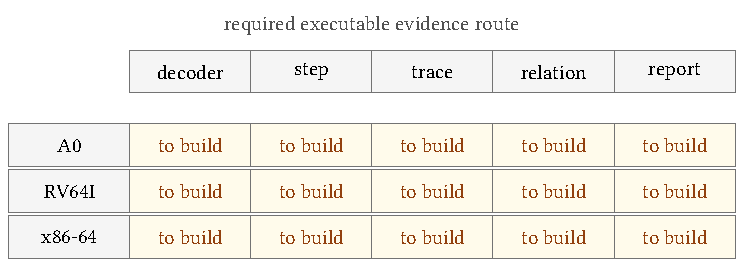
\includegraphics[width=0.94\textwidth]{figures/xor-evidence-matrix}
\caption{The case study needs separate support at the definition, execution,
relation, and certificate layers. A higher layer cannot repair a missing lower
binding.}
\figalt{Rows for A0, RV64I, and x86-64 cross columns for decoder, step, trace, relation, and evidence report; missing real-machine cells remain visibly unfilled.}
\label{fig:xor-evidence-matrix}
\end{figure}

\subsection{A staged artifact route}

The A0 package comes first because its semantics are defined by this book. A
complete package needs state types, encoder and decoder, single-step behavior,
bounded traces, range-checked little-endian memory, and controls for every
instruction used here. The XOR-reduction artifact can then execute the A0
listing and compare its terminal state with a direct fold computation.

Each real-machine package needs a pinned source boundary, decoder coverage for
the exact byte forms in its listing, and executable step semantics. The first
cross-ISA milestone is not the whole loop. It is one load, one XOR, one pointer
update, and one branch under explicit state relations. Only after those local
steps pass positive and negative controls should the route compose them into
the loop invariant.

A bounded solver query can search for a disagreement up to a chosen maximum
count and finite memory shape. If it finds one, replay it through all three
executors. If it finds none, the report supports only that bound and encoding.
The universal reader proof still depends on the stated semantic lemmas. A
future certificate route may reduce the bounded query to a checkable formula,
but it must bind formula generation to the machine definitions as Chapter 14
requires.

The evidence manifest for this example should name more than three program
files. It should bind the fold specification, precondition, observation,
machine-package versions, ABI profiles, assembled bytes, decoded listings,
initial-state constructors, trace bounds, comparison command, and controls.
The report must distinguish successful normal comparison from a trap, bound
exhaustion, decode refusal, unsupported instruction, digest mismatch, and
control failure.

Two reproduction routes are useful. The lesson route takes a short word list
and prints a human-sized trace like the table above. The artifact route consumes
raw program and memory bytes and emits a structured report. Both must invoke
the same Rust semantics. If the lesson reimplements the machines directly in
Python, agreement with the artifact might compare two subtly different
definitions.

\begin{table}[htbp]
\centering
\caption{Minimum manifest bindings for the three-machine case study.}
\begin{tabular}{@{}p{0.25\textwidth}p{0.64\textwidth}@{}}
\toprule
Binding & Question it answers \\
\midrule
Claim and scope & Which width, inputs, outcomes, and exclusions are asserted? \\
Semantics & Which A0 definition and pinned real-ISA slices interpret bytes? \\
Programs & Which raw bytes, entry addresses, and decoded instructions run? \\
Harness & How do logical inputs and successful outputs map to machine states? \\
Checker & Which command and version decide the comparison? \\
Controls & Which named mutations must the same route reject? \\
\bottomrule
\end{tabular}
\end{table}

The empty case is the best first end-to-end control because it crosses every
setup and return layer without accessing data memory. The one-word case then
fires the load and XOR paths. The two-word case fires the backward edge and
pointer update. A test plan built in this order diagnoses more than a single
large example: when a stage first fails, the newly exercised movement is
small enough to inspect.

After those concrete cases, symbolic execution can replace the word contents
with bit-vector variables. The expected result is the symbolic XOR of the
loaded variables. Symbolic addresses should wait until the range model and
alias policy are explicit; otherwise one query silently combines instruction
correctness with a much harder memory-model question.

The concrete ladder should also include values chosen for semantic edges, not
only convenient arithmetic. An all-zero word checks that XOR itself does not
manufacture bits. Repeating the same word twice checks cancellation. A word
with only the high bit set catches accidental signed reasoning. Alternating
bytes make an endian reversal visible. Placing the array at the highest valid
starting address exercises the range premise without crossing it. None of
these cases replaces the invariant, but each attacks a different connection
between the logical fold and a machine trace.

\begin{proofkit}[title={From test ladder to proof obligations}]
For each concrete case, record the semantic feature it exercises. Then replace
the particular values with variables while keeping the same precondition and
observation. The resulting obligation should explain why the case generalizes:
XOR identity, cancellation, byte reconstruction, range validity, pointer
advance, or loop progress. A test with no named obligation is useful for fault
finding but carries no clear part of the proof.
\end{proofkit}

The same ladder gives controls a deliberate order. Reverse one load's byte
join for the alternating-byte case. Change one branch predicate for the empty
case. Advance the pointer by the wrong word size for the two-word case. Remove
the memory-frame clause and show that an injected store escapes detection.
Each mutation should fail first at the relation component designed to catch
it. If a later, unrelated check fails instead, the report is too coarse or an
earlier binding is missing.

\section{What this chapter establishes, and what it does not}

The mathematical argument establishes the XOR-fold loop for the printed
logical algorithm. The instruction-level arguments explain how the selected
listings instantiate its variables and control. The cross-machine simulation
identifies the cut-point relation needed for agreement. These are reader
proofs over the semantics stated in this book and the pinned real-ISA sources.

The chapter does not yet present machine-produced Axeyum evidence for the real
listings. It does not cover optional compressed or vector instructions,
different ABIs, arbitrary misaligned accesses, concurrent memory changes,
memory-mapped input, faults outside the precondition, or timing. It does not
claim the listings are minimal or fastest. Those exclusions are part of the
result's meaning.

The example also marks a transition in scale. We have moved from one
instruction to a loop and from one state relation to three executions. Yet the
method did not change: define the words, inventory the state, state the
observation, prove a local movement, compose movements at named cut points,
and bind any machine-derived evidence to the exact claim.

\section{Exercises}

\begin{enumerate}
\item \textbf{Execute.} Trace all three logical iterations in the table from
the byte contents of memory, showing each little-endian reconstruction.
\item Trace the A0 listing for \(n=0\). Name every executed address and explain
why no data-memory read occurs.
\item Compute the two A0 branch displacements from the printed addresses and
reconstruct both targets from the encoded values.
\item State the loop invariant after the load but before XOR. Which additional
temporary value must it name?
\item Prove that XOR reduction is unchanged by swapping two adjacent input
words. Explain why that is a weakness for a security checksum.
\item Prove that appending the current reduction value to a region makes the
new reduction zero.
\item \textbf{Break.} Change the pointer increment from eight to four. Give the
smallest count and memory bytes that separate the programs.
\item Change the A0 backward branch displacement from \(-5\) to \(-4\). Trace
the first two visits to the resulting target.
\item Delete the RV64 empty-input branch. Give an input allowed by the original
contract that now fails, and classify the failure.
\item Replace x86 \code{xor eax,eax} with a write to \code{ax}. Explain which
initial register values expose the subregister error.
\item Write the complete read and write sets for one loop body on each machine,
including program counter and condition state.
\item Define a relation between the A0 state after \code{load} and the RV64
state after \code{ld}. Include the temporary loaded word.
\item \textbf{Prove.} Expand the body-correspondence paragraph into one lemma
per instruction group, with precondition and postcondition for each lemma.
\item Strengthen the observation to require scratch registers to agree. Show
why the printed three-way theorem then fails or becomes unnatural.
\item Weaken the observation by dropping memory preservation. Construct a
program that returns the right result while corrupting one input byte.
\item Change the specification from XOR reduction to modular sum. Identify the
parts of the invariant and listings that change, and the parts that remain.
\item Add a stride \(s\) to the contract. State sufficient no-wrap and readable-
range premises for addresses \(a+si\).
\item Permit \(n\) to use every 64-bit unsigned value. Explain why termination
in natural-number arithmetic still needs an address and resource story.
\item Design one positive and four negative controls for the future Axeyum A0
artifact. Name the expected outcome class of each.
\item Design a bounded disagreement query for counts at most three. List its
symbolic inputs, transition constraints, observation, and replay requirement.
\item \textbf{Transfer.} Rewrite the routine for a different calling convention.
Separate instruction semantics from the new register and preservation rules.
\item Compare a scalar XOR reduction with a vector version conceptually. List
the additional state, instruction, and reduction-order questions that move the
vector proof beyond this chapter's model.
\end{enumerate}
